\section{Experimentation and Results} 
%\subsection{Overview} 
\begin{figure}[htbp] %  figure placement: here, top, bottom, or page
   \centering
   \includegraphics[width=17cm]{images/Architecture3.pdf} 
   \caption{Component view of the Architecture}
   \label{fig:SysArc}
\end{figure}

Figure~\ref{fig:SysArc} shows the component view of our proposed system architecture. It is similar to the one proposed in \cite{1}.
It is divided into two parts: An \textit{Environment Model} which stores the information about the environment and a \textit{Navigation Planning System} 
which uses the environment information to generate navigation plans.
They are both indicated by grey color blocks in the Figure~\ref{fig:SysArc}. The dotted boxes are assumed to be existing/working in the system. 
The \textit{Navigation Planning System} is further divided into three components: Semantic Navigation Planner, Navigation Knowledge base and Navigation Failure Diagnosis.
The sections below explain both parts of our architecture in detail starting with the \textit{Environment Model} and then the \textit{Semantic Navigation Planner}.\\

We consider the home environment setup of scenario 2 mentioned in section~\ref{sec:har} for explaining the architecture. 
It is assumed that the present location of the robot is \textit{livingroom-1} and it gets the goal of ``go to kitchen" from the symbolic(task) planner.  

%\subsection{Environment model}

This section elaborates our combined map which represents spatial and semantic knowledge of the environment.

\begin{figure}[htbp] %  figure placement: here, top, bottom, or page
   \centering
   \includegraphics[width=15cm]{images/semanticMap1.pdf} 
   \caption{Block diagram of our \textit{Environment model}}
   \label{Figure: Block diagram of our Environment model}
\end{figure}

Our model represents metric, topological and semantic features of the environment in two separate parts \cite{2}:  S-Box (spatial box) and T-Box (terminological box).
This representation methodology is adopted from the approaches \cite{2, 3, 4, 5, 6} which are mentioned in detail in section~\ref{sec:semantics} .\\

The S-Box represents spatial and symbolic information. 
Spatial information of the entities(\textit{regions} and \textit{objects}) in the environment is stored at the lower level. 
These entities are assigned symbols(labels) which form the top level of S-Box. 
T-Box stores the meaning(semantics) of these entities in the form of concepts and their relations.
In this work, we consider two concepts to represent the environment information: \textit{Regions} and \textit{Objects}.
Symbols in S-Box are instances of these concepts in T-Box.
For instance, considering the home environment setup, the lower level of S-Box may store the metric(occupancy grid) map of a kitchen. This map is assigned a symbol, say, \textit{kitchen-1} and stored at the symbolic (top) level of S-Box.
T-Box would then store the semantic information that kitchen is a type of \textit{Region} and implies a space with some properties and contains objects like fridge, oven, stove etc.

\subsubsection{S-Box}
\begin{figure}[htbp] %  figure placement: here, top, bottom, or page
   \centering
   \includegraphics[width=14cm]{images/sboxexample.pdf} 
   \caption[S-Box of our \textit{Environment Model}]
   {S-Box of our \textit{Environment Model}. Here only connections for room1 and object1 with other levels are shown. 
   Same connections exist for all rooms and objects.
   Bold line indicates separation between two levels of information. Dotted line indicates the layers are at the same level}
   \label{fig:Our Semantic map}
\end{figure}

Information in S-Box is stored in two levels: Spatial level and Symbolic level.\\
This forms a spatio-symbolic hierarchy \cite{3} since the symbolic level is formed over the spatial level.\\\\
Spatial level represents spatial information in four different layers\cite{2, 7}:
\begin{itemize}
 \item \textit{Appearance layer}
 \item \textit{Occupancy layer}
 \item \textit{Navigation layer}
 \item \textit{Topological layer}
\end{itemize}
However, these layers do not form a hierarchical representation. In fact, they are arranged in series 
forming a flat representation. This representation is adopted in order to keep the layers (of spatial level) independent 
of each other, so that if a domain does not require any of these layers, it could be omitted easily without affecting the system. \\

At the symbolic level, instances (symbols) of entities are maintained in one single layer. We term this layer as \textit{Symbolic layer}.  
The \textit{Appearance, Metric, Navigation} and \textit{Topological} layers of the spatial level are each individually linked to the \textit{Symbolic layer} as shown in Figure~\ref{fig:Our Semantic map}. 
For instance, in the figure, the local grid map-1 of the doorway is connected to its instance \textit{doorway-1} at the symbolic level. 
Similarly, the semantic position of this doorway at the navigation level and its node(region-1) at the topological level are connected to its instance \textit{doorway-1}.
Also, as indicated in the figure by dotted bi-directional arrows, this linking provides inferencing in both the directions \footnote[4]{Inferencing in both directions: If our model is queried for instances of kitchen, it will give \textit{kitchen-1} as the answer. 
Also, if the model is queried to which class the symbol \textit{kitchen-1} belongs to, it will give the answer as kitchen}.

\paragraph{Appearance layer}
The \textit{Appearance layer} stores information about the objects in the environment.
It could be object images or pound cloud data obtained from sensors.
However, the focus of this work is on representing information about spatial entities and using the same for navigation.
Hence, we do not go into the details of representing objects in the environment. 
The layer could be considered to be non-existing for this work and could be substituted by any appropriate representation, 
depending on the domain requirement.

\paragraph{{Metric layer}}
The \textit{Metric layer} stores spatial information in the form of local grid-maps with respect to local coordinate system.
These local grid-maps are a representation of the regions existing in the environment.
Longer sides of the regions face towards north in their local coordinate system \cite{1} as shown in the Figure~\ref{fig:cs} below:\\ 
\begin{figure}[htbp] %  figure placement: here, top, bottom, or page
   \centering
   %\includegraphics[angle=90,width=10cm]{images/tbox.jpg}
   \includegraphics[width=9cm]{images/metriclayer.pdf}
   \caption{Definition of local coordinate system for regions based on \cite{1}} 
   \label{fig:cs}
\end{figure}\\
This layer also maintains the shape of the regions representing the geometric area covered by the regions with respect to a global coordinate frame.
The shape of the regions is represented using the method used in \cite{1} where a center rectangle is used along with two connected sub-rectangles as shown in Figure~\ref{fig:geo} below. 
\begin{figure}[htbp] %  figure placement: here, top, bottom, or page
   \centering
   %\includegraphics[angle=90,width=10cm]{images/tbox.jpg}
   \includegraphics[width=9cm]{images/geometry.png}
   \caption[Region geometry represented by triple \cite{8}]
   {Region geometry represented in \cite{8} by triple \textit{(x, y, w, h, $\theta$, $w_{l}$, $h_{l}$, $y_{l}$, $w_{r}$, $h_{r}$, $y_{r}$)}} 
   \label{fig:geo}
\end{figure}

\paragraph{{Navigation layer}}
This layer basically maintains navigable points of a region.
Each region has a navigation point which we call as \textit{semantic position} associated with it \cite{8}.
Regions can have multiple semantic positions as well. 
Even stationary objects like fridge or doors can have \textit{semantic positions}. Robots usually have to manipulate objects like doors,
or they need to go close to 
objects like table for grasping objects like coffee cups kept on the table . 
Semantic positions associated with such objects(doors, tables) would help to serve the purpose of manipulating and/or grasping better.
Even movable objects(like cups) can have semantic positions which would help in grasp planning as mentioned in \cite{18}. 
Our work considers only semantic positions associated with regions.\\

As shown in the Figure~\ref{fig:Our Semantic map} , the semantic positions are encircled indicating their belonging to a particular region. For instance, for \textit{livingroom-1} two semantic positions are encircled: one for the room itself to help the robot to navigate to the living room 
and one for \textit{table-1} to help the robot to grasp some other object placed on the table. The details of semantic positions is elaborated in section ~\ref{sec:semanticposition} .

\paragraph{{Topological layer}}
The \textit{Topological layer} represents topological connectivity between \textit{Regions}.
\textit{Regions} are represented by nodes, like in Figure~\ref{fig:Our Semantic map} , doorway-1 is represented by node \textit{region1}. 
Edges connecting the nodes represent the relation \textbf{neighbourOf} which indicates that \textit{Regions} are topologically connected to their neighbors \cite{1}.
Also, the relative orientation of neighbouring regions is represented in the layer using the concepts: \textbf{northOf, eastOf, southOf} and \textbf{westOf} \cite{1}. The relationships are shown in Figure~\ref{fig:r}.  
\begin{figure}[htbp] %  figure placement: here, top, bottom, or page
   \centering
   %\includegraphics[angle=90,width=10cm]{images/tbox.jpg}
   \includegraphics[width=8cm]{images/topologicallayer.pdf}
   \caption[Topological relations between regions based on \cite{1}]
   {Topological relations based on \cite{1}: C represents \textit{Region} concepts and R their relations}.
   %\textit{Note: Italic text indicates concepts and bold text indicates their relations}} 
   \label{fig:r}
\end{figure}
Maintaining such relationships makes human-robot communication more effective by helping humans in assigning tasks to robot or retrieving information about the robot status in large environments \cite{8}.
For instance, robots could be given a task \textit{``Bring `x' book from the room which is to the north of room `y' "}.
Or the robot can inform the operator \textit{``I am stuck in the corridor which is to the east of room `z' "}.\\

The topological layer  could be viewed as a layer dividing the semantic positions in the navigation layer into regions,
for instance, in the Figure~\ref{fig:Our Semantic map} , region2 represents a region consisting of two semantic positions.
For navigation planning, the topological connectivity between regions helps the planner to generate a symbolic plan which consists of regions the robot
has to navigate through to reach the goal. Based on this symbolic plan, the semantic navigation planner further queries the environment model for the corresponding semantic positions
For instance, if the robot is in the \textit{livingroom-1} and has go to \textit{kitchen-1}, the planner first queries the topological layer about the connectivity between these two regions ({\textit{livingroom-1 $\longleftrightarrow$ doorway-2 $\longleftrightarrow$ kitchen-1}})
and then based on this information, the planner queries the navigation layer for semantic positions of these regions.

\paragraph{{Symbolic layer}}
At this layer, entities in the environment are represented in the form of symbols(labels).
These symbols are instances of concepts(\textit{Region} and \textit{Object}) in T-Box.
%Maintains environment information in the form of instances of entities (\textit{Region} and \textit{Object}).
%An instance of a new entity is created by asserting a unique symbol(label) to it and linking this symbol to the corresponding concept (in T-box).
Whenever an instance of a new entity is created it is linked to its corresponding concept in T-box by assigning a unique symbol to it and asserting this symbol to the corresponding concept in T-box.
%Lower layers basically maintain metric, topological and semantic properties of these instances.
For instance, suppose a new local grid map of a region, say, living room is created. This map is be asserted a symbol \textit{livingroom-1} and
is linked to the concept \textit{Region} (or \textit{LivingRoom} to be precise, which is a sub-category of \textit{Region}) in the T-Box. 
Similarly, the semantic positions and topological relations are asserted to the symbol of the new entity created. 
This process of assertion and linking could be done by hand(by a human operator) while creating the environment representation using some knowledge representation language \footnote[5]{In \cite{2} LOOM knowledge representation system\cite{24} is used to create the concepts and relations of the T-Box.
In \cite{3, 4} NeoClassic system\cite{25} is used to create concepts and the linking between the sensor data(grid map) and symbols is done using a process called Anchoring \cite{23}. \cite{22, 17} uses Web Ontology Language(OWL)\cite{26} while \cite{1} uses ObjectLogic\cite{27}}.
It could also be taken care of by an on-line SLAM algorithm, like the one proposed in \cite{8} which is capable of creating an environment representation with semantic, metric and topological features.\\

Although the focus of this work is not on representing object entities, for now,we group symbols of objects based on their geometric positions and 
use human-like environment distribution(that is, objects \textit{are located} in rooms)\cite{3}.
For instance, in Figure~\ref{fig:Our Semantic map} , objects(\textit{tvset-1, plant-1} etc) belonging to the living room are grouped together and linked to \textit{livingroom-1} symbol via \textbf{at} relation.
However, different criteria could be used depending on the application. For instance, objects could be grouped based on their mobility \cite{21, 22}.\\
\textit{Example:} Structural objects(walls,floors) could be grouped together, while furniture objects
(table, chair etc) will form another group.


\subsubsection{T-Box}
\begin{figure}[htbp] %  figure placement: here, top, bottom, or page
   \centering
   %\includegraphics[angle=90,width=10cm]{images/tbox.jpg}
   \includegraphics[width=10cm]{images/tbox3.pdf}
   \caption{\textit{Region} and \textit{Object} concept and their relation}
   \label{fig:T-Box}
\end{figure}
\begin{figure}[htbp] %  figure placement: here, top, bottom, or page
   \centering
   %\includegraphics[angle=90,width=10cm]{images/tbox.jpg}
   \includegraphics[width=15cm]{images/tbox1.pdf}
   \caption{Extension of \textit{Region} concept}
   \label{fig:TBox2}
\end{figure}
\begin{figure}[htbp] %  figure placement: here, top, bottom, or page
   \centering
   %\includegraphics[angle=90,width=10cm]{images/tbox.jpg}
   \includegraphics[width=12cm]{images/tbox2.pdf}
   \caption{Extension of \textit{Object} concept}
   \label{fig:TBox1}
\end{figure}
The T-Box stores semantic knowledge about the robot environment. 
We refer to this knowledge as semantic because it assigns meaning to the information represented in the S-Box.
The knowledge includes the types of entities(regions and objects) found in the environment along with their relationships.
It is represented in the form of concepts and relations which are structured in hierarchical form called ontology \cite{2}.
Our ontology consists of two concepts: \textit{Region} and \textit{Object} which are related by \textbf{located-at} relation 
as shown in Figure~\ref{fig:T-Box} .
Further sub categorization of \textit{Region} and \textit{Object} concepts is done until reaching most specific categories like 
\textit{kitchen, living room, office room} etc.
%For this work the focus is on representing spatial properties of regions in the environment to help plan navigation. So the \textit{Object} concept is not elaborated in detail in the ontology. 
% (But the representation will be flexible to incorporate as many Object categories and properties  as required by the application domain) 
Since the focus of this work is on navigation we consider detailed categorization of \textit{Region} which is shown in Figure~\ref{fig:TBox2} ,
considering two different environment setups (Home and University) mentioned in section~\ref{sec:har}.
Also, general categorization of \textit{Object} concept is shown in Figure~\ref{fig:TBox1} .\\

Along with representing the entities and their relations in hierarchical form(ontology), the T-Box also stores general knowledge about them by
assigning meaning to concepts(entities) in the ontology.
For instance, the T-Box stores the information that \textit{Kitchen} is a \textit{Room} containing a \textit{Fridge} and \textit{Stove}. 
This is depicted in the Figure~\ref{fig:SM} :

\begin{figure}[htbp] %  figure placement: here, top, bottom, or page
   \centering
   %\includegraphics[angle=90,width=10cm]{images/tbox.jpg}
   \includegraphics[width=4cm]{images/tbox4.pdf}
   \caption{Definition of \textit{Kitchen} concept in T-Box}
   \label{fig:SM}
\end{figure}

\paragraph{Our T-Box ontology}
As mentioned above, the focus is on the concept \textit{Region}.
The \textit{Region} concept is categorized into: \textit{Room, Passage, Corridor} and \textit{Junction}.
\begin{itemize}
 \item \textit{Room:} This concept is further sub-categorized into concepts like \textit{Kitchen}, \textit{Living room}, \textit{Office room} and other types 
 of rooms found in human environment.
 \item \textit{Passage:} This concept represents regions which help the robot to transit from one region to other. The concept \textit{Passage} is further categorized into:
 \begin{itemize}
  \item \textit{Horizontal Passage} which includes \textit{Doorway} (and \textit{Window}).
  \item \textit{Vertical Passage} is further categorized as \textit{Elevator}.
 \end{itemize}
The reason for treating \textit{Doorway}, \textit{Elevator} different from \textit{Room} is to help navigation planner adopt different strategies (if required) 
while navigating through narrow doorways, elevators. 
This also helps in reasoning and recovering in case of failure while navigating through the doorways, elevators . 
 \item \textit{Corridor:} This concept represents long regions connecting different rooms.
 \item \textit{Junction:} In this work we introduce a new concept called \textit{Junction} to deal with situations, where two or more corridors intersect. 
Such a region is called a \textit{Junction} in our approach.
Figure~\ref{fig:jn} shows an example:
\begin{figure}[htbp] %  figure placement: here, top, bottom, or page
   \centering
   %\includegraphics[angle=90,width=10cm]{images/tbox.jpg}
   \includegraphics[width=6cm]{images/tbox5.pdf}
   \caption{\textit{Junction} concept example}
   \label{fig:jn}
\end{figure}
\end{itemize}


\iffalse 
\subsubsection{ Semantic SLAM:}
\begin{itemize}
 \item This work will make use of SLAM approach similar to the one developed in \cite{8}.
 \item The approach uses FastSLAM 2.0 capturing region features with semantic, topological as well as metric properties.
 \item It assigns semantic meaning to the regions (e. g., rooms, offices,hallways, doors, desks, cupboards, etc.), and also assign topological relation between these regions as well as maintain 
 geometric layout of each region.
 \item \textit{Semantic description:} Includes the type of the sub-category of the region class to which the region under consideration belongs to. To deal with uncertainity, a confidence value is assigned.
 \item In this work, we include additional information at the semantic level. This includes adding semantic positions to each instance of region class. Figure 6 depicts the semantic description part of the data structure with addition of semantic position. 
 \item \textit{Topological description:} Connectivity to the neighboring regions and also hierarchical links to sub-regions. The connectivity is associated with a confidence value to deal with uncertainity.
 \item \textit{Geometric description:} Regions' geometric is modeled by three rectangles along horizontal axis. The entire shape could be rotated arbitrarily. Shown in figure 7.

 \item Figure below shows the representation used in \cite{8} to store the region features.
  \begin{figure}[htbp] %  figure placement: here, top, bottom, or page
    \centering
    %\includegraphics[angle=90,width=10cm]{images/tbox.jpg}
    \includegraphics[width=10cm]{images/SLAM.png}
    \caption{Storing semantic, topological and metric features \cite{8}}
    \label{Fig:} 
  \end{figure} 
  \begin{figure}[htbp] %  figure placement: here, top, bottom, or page
    \centering
    %\includegraphics[angle=90,width=10cm]{images/tbox.jpg}
    \includegraphics[width=10cm]{images/semanticposition.png}
      \caption{Semantic description part after addition of semantic position details}
    \label{Fig: Semantic description part after addition of semantic position details}
  \end{figure} 
\end{itemize}
\begin{figure}[htbp] %  figure placement: here, top, bottom, or page
   \centering
   %\includegraphics[angle=90,width=10cm]{images/tbox.jpg}
   \includegraphics[width=10cm]{images/geometry.png}
   \caption{}
   \label{Fig: Method of storing geometric shape of the room}
\end{figure}
\fi
%\subsection{Semantic positions}
\label{sec:semanticposition}
\subsubsection{Representing Semantic positions}
This work represents semantic positions associated with regions by three properties namely:
  \begin{itemize}
    \item \textit{Location}
    \item \textit{Orientation} 
    \item \textit{Tolerance} 
  \end{itemize}
\textit{Location} and \textit{Orientation} concepts are adopted from the approach in \cite{1}, while the \textit{Tolerance} concept is the contribution of this work.
The \textit{Location} and \textit{Orientation} properties are concerned with the x-y co-ordinate of the robot and its rotation angle with respect to local reference frame of that region.
The \textit{Tolerance} property determines how close the robot is expected to go to the semantic position.\\

These properties are represented by symbols and not by numerical values \cite{1}.
The instances of symbols for \textit{Location, Orientation} and \textit{Tolerance} properties used in this work are mentioned below:
\begin{itemize}
  \item \textit{Location} of SP: center/east/west/north/south/north-east/north-west/south-east/south-west
  \item \textit{Orientation} of SP: east/west/north/south
  \item \textit{Tolerance} for SP: soft/medium/hard
\end{itemize}
An example of a semantic position for \textit{kitchen-1} instance of our home environment setup is shown below:
\begin{itemize}
  \item \textit{Location}: center
  \item \textit{Orientation}: north
  \item \textit{Tolerance}: soft/medium/hard
\end{itemize}
The definitions/equations of these symbols are stored in the \textit{Navigation Equations component} of the architecture elaborated in section~\ref{sec:ne} .
However, depending on the application domain, the symbols could be added/removed/modified along with their definitions in the \textit{Navigation Equations component}.\\

Usually rooms and other categories of \textit{Region} concept will have soft or medium tolerance.
\textit{Objects} will mostly have hard tolerance.
These assumptions may change depending on the application domain.

\subsubsection{Advantage of \textit{Tolerance} limit} 
\textit{Tolerance} limit for a semantic position makes navigation flexible in the following way:
Usually a robot goes to a room and then proceeds towards some object.
For instance, in our home environment setup, suppose the robot is given the task of ``bringing a milk bottle". The robot needs to go to the
kitchen and dock a fridge to pick-up the milk bottle. In such scenarios, the robot does not need to reach the exact semantic position of the kitchen.
%it is acceptable if the robot does not exactly reach the kitchen's semantic 
%position since there its is not expected to manipulate any object. Instead it has to approach the fridge after entering the kitchen. 
Assigning soft tolerance to the semantic position of the kitchen enables the robot to conclude the accomplishment
of the goal of ``going to kitchen"  as soon as it is in the kitchen.\\

For the same task, after reaching the kitchen the robot has to dock the fridge to grasp a milk bottle. Hence, fridge could have medium tolerance limit indicating
that robot has go near to the fridge. This nearness depends on the workspace of the robot platform. A hard tolerance limit indicates that the robot has to be at the exact position.
Assigning a hard or soft tolerance limit to the semantic position of an object depends on the workspace of the robot. Robots with limited workspace need to
have hard tolerance to grasp objects. However, regions can always have a soft tolerance limit, irrespective of the platform workspace,
unless robots are not grasping any objects at those positions.\\

The tolerance limit helps to deal with situations in which dynamic obstacles in the vicinity or on the semantic positions. 
It also improves the path planning efficiency by reducing the goal completion time.
%\subsection{Navigation Planning System}
\begin{figure}[htbp] %  figure placement: here, top, bottom, or page
 \centering
   %\includegraphics[angle=90,width=10cm]{images/tbox.jpg}
   \includegraphics[width=23.6cm, height=13cm, angle=90]{images/snp_1backup.pdf}
   \caption{Navigation Planning System}
   \label{Fig: Method of storing geometric shape of the room}
\end{figure}
We consider an example in the home environment setup of scenario 2 mentioned in section~\ref{sec:har}  for explaining the system. 
In this example, the robot gets a symbolic goal of ``go to kitchen" from the high 
(task/symbolic) level planner. Let us assume the current semantic location of the robot 
as ``living room".

\subsubsection{Overview}
The system works in three stages:
\begin{itemize}
 \item Planning: At this stage the navigation is planned by dividing the symbolic goal received from the high level (task) planner into an array of geometric sub-goals.
 \item Monitoring: This stage feeds the geometric sub-goals to the motion planner and monitors its execution.
 \item Recovery: This stage is initiated if the robot is not able to achieve its goal/sub-goal. At first the cause of failure is identified and then the necessary recovery is conducted.
\end{itemize}

The \textit{Navigation Planning System} gets its goal ``go to kitchen" from the high level 
(task / symbolic) planner.
The \textit{Environment model} is then queried about the robot's current semantic position which in this case is the \textit{living room-1}.
Accordingly, the system generates a semantic navigation plan consisting of a set of sequential symbolic sub-Version1goals.
In this example, the semantic navigation plan is: ``go to \textit{doorway-1}", ``go to \textit{kitchen-1}".
Once this abstract plan is generated, the planner system queries the \textit{model} again, this time asking for corresponding semantic positions associated with these region instances (\textit{doorway-1, kitchen-1}).
These semantic positions are then fed to the motion(path) planner in a sequence.
If the robot is not able to reach its goal/sub-goal (\textit{kitchen-1}), the planning system searches for the cause (may be blockage of \textit{doorway-1} due to malfunctioning of \textit{door-1})
and accordingly modifies the plan to achieve the goal.
If the goal is not achieved even after executing all possible/relevant recovery options, the planner sends a failure notification along with the cause
to the high level planner.\\

Sections below explain working of each component of our proposed system. Figure~\ref{fig:legend} gives the meaning of the symbols used to explain component.
\begin{figure}[htbp] %  figure placement: here, top, bottom, or page
   \centering
   %\includegraphics[angle=90,width=10cm]{images/tbox.jpg}
   \includegraphics[width=6cm]{images/snp_legend.pdf}
   \caption{Legend for Navigation Planning System of Figure~\ref{Fig: Method of storing geometric shape of the room}}
   \label{fig:legend}
\end{figure}

\subsubsection{Plan Generator}
\begin{figure}[htbp] %  figure placement: here, top, bottom, or page
   \centering
   %\includegraphics[angle=90,width=10cm]{images/tbox.jpg}
   \includegraphics[width=12cm]{images/snp1_1.pdf}
   \caption{Plan Generator component}
   \label{Fig:Data flow summery}
\end{figure}
This is the component where actual navigation plans are generated for the motion(path) planner.
It gets a symbolic navigation goal from a high level (task/symbolic) planner, for instance, ``go to \textit{kitchen-1}".
Once it gets a goal, it queries the \textit{Localization cache} about robot's current semantic position (\textit{living room-1} in our example).
Then it queries the \textit{Environment Model} via the \textit{Map cache} component to get the topological connectivity between 
the robot's current semantic position(\textit{living room-1}) and the semantic goal(\textit{kitchen-1}).
This symbolic goal is then divided into symbolic sub-goals (``go to \textit{doorway-1}", ``go to \textit{kitchen-1}") based on the response 
from the \textit{Environment Model}.
Further, the semantic positions of these subgoals are queried(to the \textit{Environment Model} via the \textit{Map cache}) and a sequence of geometric sub-goals i.e semantic positions with constraints, is generated. 
Each sub-goal has a set of constraints which could be geometric, kinematic, dynamic or semantic. 
This work considers only semantic and dynamic constraints.
Semantic constraints include tolerance limit associated with each semantic position.
For dynamic constraints we consider robot velocity and acceleration.
Once a set of sequential (geometric) sub-goals with constraints is generated, it is fed to the next component, that is, the \textit{Scheduler}.  

\subsubsection{Scheduler}
\begin{figure}[htbp] %  figure placement: here, top, bottom, or page
   \centering
   %\includegraphics[angle=90,width=10cm]{images/tbox.jpg}
   \includegraphics[width=5cm]{images/snp2.pdf}
   \caption{Scheduler component}
   \label{Fig:Data flow summery}
\end{figure}
The \textit{Scheduler} component is a data base which maintains the sub-goals in a sequential manner as generated by \textit{Plan Generator} component.
It also stores the associated constraints for each sub-goal as shown in the Figure ~\ref{fig:s} .
In our example, sub-goal $g_{1}$ is the semantic position associated with \textit{doorway-1} and $g_{2}$ is semantic position for \textit{kitchen-1}.
$c_{1}, c_{2}$ as indicated in the figure are the constraints: {tolerance limit, velocity, acceleration}. 
Each sub goal is fed to the motion(path) planner through the \textit{Monitor Unit}, upon receiving the previous goal completion notification. 
For instance, once the sub-goal $g_{1}$ is fed to the motion(path) planner (through the \textit{Monitoring} component), the \textit{Scheduler} will wait for a response from 
the \textit{Monitoring} component about completion of sub goal $g_{1}$ before sending the next sub goal $g_{2}$.

 \begin{figure}[htbp]
 \centering
 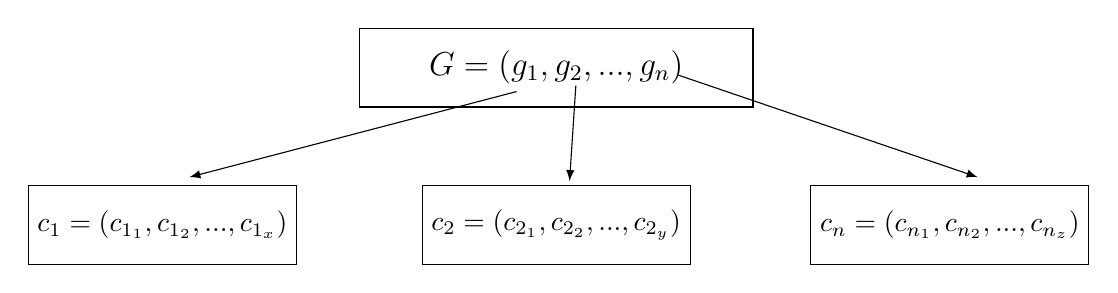
\begin{tikzpicture}
% two boxes
\node[draw,minimum width=5cm, minimum height=1cm] (a) at (5,0) {\large $G = (g_{1} ,  g_{2} ,...,  g_{n})$};
\node[draw,minimum width=3cm, minimum height=1cm] (b) at (0,-2) {$c_{1} = (c_{1_1},c_{1_2},...,c_{1_x})$};
\node[draw,minimum width=3cm, minimum height=1cm] (c) at (5,-2) {$c_{2} = (c_{2_1},c_{2_2},...,c_{2_y})$};
\node[draw,minimum width=3cm, minimum height=1cm] (d) at (10,-2) {$c_{n} = (c_{n_1},c_{n_2},...,c_{n_z})$};

\path (a.east) -- (a.south west) coordinate[pos=0.6] (a1);
\path (b.west) -- (b.north) coordinate[pos=1.2] (b1);
\draw[latex-] (b1) -- (a1);

\path (a.east) -- (a.south west) coordinate[pos=0.45] (a2);
\path (c.west) -- (c.north) coordinate[pos=1.1] (b2);
\draw[latex-] (b2) -- (a2);

\path (a.east)  -- (a.south west) coordinate[pos=0.19] (a3);
\path (d.west) -- (d.north) coordinate[pos=1.2] (b3);
\draw[latex-] (b3) -- (a3);
\end{tikzpicture}
 \caption[Symbolic goal, geometric subgoals and constraint lists]
 {G is the symbolic goal which is segmented into geometric subgoals of $g_{1},...,g_{n}. c_{1}...c_{n}$ represents associated list of constraints}
 \label{fig:s}
\end{figure}

\subsubsection{Monitoring}
\begin{figure}[htbp] %  figure placement: here, top, bottom, or page
   \centering
   %\includegraphics[angle=90,width=10cm]{images/tbox.jpg}
   \includegraphics[width=12cm]{images/snp3.pdf}
   \caption{Monitoring component}
   \label{Fig:Data flow summery}
\end{figure}

The purpose of this component is twofold:
  \begin{itemize}
   \item The \textit{Monitoring} component acts as a coordinator between the \textit{Scheduler} and the motion(path) planner.
   \item Monitoring the working of the motion planner while it attempts to reach the given goal/sub goal.
\end{itemize}
The \textit{Monitoring} component queries the \textit{Scheduler} for a subgoal(with constraints) and 
sends it to the motion planner depending on its status(whether the planner is free).
It then monitors the motion(path) planner executing the given subgoal.
The motion planner notifies the \textit{Monitoring} component about the completion of the sub goal by firing an event.
The motion planner triggers a failure event if the previous sub goal is not achieved, notifying the \textit{Monitoring} component about the failure.
In situations of failure the \textit{Monitoring} component informs the \textit{Navigation Failure Diagnosis} unit.\\

Another important function the \textit{Monitoring} component is expected to perform is setting appropriate parameters\footnote[6]{ROS Navigation stack consist of a set of parameters for (global and local) planners which could be set to customize the behavior of the planners. \url{http://wiki.ros.org/navigation/Tutorials/RobotSetup}. [Online]. Accessed: Oct. 22, 2013] } 
for the motion planner to satisfy the given constraints. 
However, this might not be necessary for some constraints.
For instance, in our work the tolerance limit constraint associated with semantic positions has a different role to play.
It is used for the purpose of monitoring and helps in deciding when to conclude that the given subgoal is achieved.
Hence, the constraint of tolerance limit is not set by the \textit{Monitoring} component.

\subsubsection{Navigation Equations}
\label{sec:ne}
\begin{figure}[htbp]
 \centering
 \includegraphics[width=8.5cm]{images/snp4.pdf}
 \caption{Navigation Equation component}
 \label{Fig:Data flow summery}
\end{figure}

As the name suggests, \textit{Navigation Equations} component contains a set of equations(rules) which can perform certain calculations \cite{1,21}.
The calculations are performed on the properties of the \textit{semantic positions}, that is on \textit{Location, Orientation} and \textit{Tolerance}
properties which have symbolic values.
Example: \textit{Tolerance} can have symbolic values such as \textit{soft/medium/hard}.
These symbolic values are fed as input to the \textit{Navigation Equations} component which performs calculations on them
to convert them into appropriate numerical values.
For instance, if semantic position of \textit{kitchen-1} has a symbolic value \textit{center} for \textit{Location}, then 
these values are fed to the \textit{Navigation Equations} component. 
The component returns a numerical value for the symbolic value \textit{center} using the equation mentioned below:\\

\begin{center}
\begin{Large}
$ x_{center} = \frac{ w_{l} + x + w_{r} }{2}$
 
$y_{center} = \frac{ h_{l} + h + h_{r} }{2}$
\end{Large}
\end{center}

 \begin{figure}[htbp]
 \begin{center}
 \includegraphics[width=10cm]{images/geometry.png}
 \caption[Navigation equation example(up). Region geometry(down) represented by triple \cite{8}]
 {Navigation equation example(up). Region geometry(down) represented by triple $G_{R}$=\textit{(x, y, w, h, $\theta$, $w_{l}$, $h_{l}$, $y_{l}$, $w_{r}$, $h_{r}$, $y_{r}$)} \cite{8}} 
\label{Fig:Data flow summery}
\end{center}
\end{figure}

Similar equations exist for other symbolic values of \textit{Location} and for other properties of semantic positions.
These symbolic values and their definitions could be changed depending on the domain. 
Maintaining equations in a separate component helps to reduce the complexity of the system by decreasing the number of facts to be stored explicitly in the map \cite{1}.
\subsubsection{Map cache}
\begin{figure}[htbp]
 \centering
 \includegraphics[width=12cm]{images/snp5.pdf}
 \caption{Map cache component}
 \label{Fig:Data flow summery}
\end{figure}

The \textit{Map cache} temporarily maintains the environment information relevant for the navigation task being executed.
For instance, in our example, the \textit{Map cache} component maintains occupancy grid maps of \textit{livingroom-1, doorway-1, kitchen-1} along with their topological connectivity.
It also maintains their semantic positions.
Other units like the \textit{Semantic Navigation planner} or \textit{Navigation Failure Diagnosis}  query the \textit{Map cache} 
component for environment information. 
For the first time, the \textit{Map cache} queries the \textit{Environment Model} about environment information, after receiving a request about it from the \textit{Navigation planner} component.\\
This information is then maintained by the \textit{Map cache} either until the symbolic goal is achieved or till a new request is generated by the \textit{Navigation planner} component.
If some additional information is required while execution, for instance by the \textit{Navigation Failure Diagnosis} unit while dealing with unexpected situations(failures), 
it is queried to the \textit{Environment model} via the \textit{Map cache} component.

\subsubsection{Localization cache}
\begin{figure}[htbp]
 \centering
 \includegraphics[width=12cm]{images/snp6.pdf}
 \caption{Localization cache component}
 \label{Fig:Data flow summery}
\end{figure}

The \textit{Localization cache} component maintains a constant update of the robot's current location 
(semantic+topological+metric).
It gets its input from the on-line SLAM algorithm.
%Based on this it will calculate the average probability of location.
The \textit{Monitoring} and other components query the\textit{ Localization cache} for the robot's current semantic location.

\subsubsection{Navigation Failure Diagnosis(\textit{Reasoning and Recovery})}
\begin{figure}[htbp]
 \centering
 \includegraphics[width=12cm]{images/snp7.pdf}
 \caption{Navigation Failure Diagnosis Unit}
 \label{Fig:Data flow summery}
\end{figure}
During the execution of the given sub-goal, if there is a failure,
it is notified to the \textit{Navigation Failure Diagnosis} unit by the \textit{Monitoring} component by triggering a failure event.
The \textit{Navigation Failure Diagnosis} unit then takes control over the low level planners\footnote[7]{Low level planners include the global planner at the motion planning level and the local planner at the controller level as shown in Figure~\ref{fig:SysArc}} 
to overcome the situation.
While the \textit{Navigation Failure Diagnosis} unit is trying to overcome the unexpected situation, it notifies the \textit{Monitoring }component to wait until the recovery is done.
If no solution works for recovering from the situation, the high level (task/symbolic) planner is notified about the symbolic goal failure. \\

However, Failure Diagnosis and Reasoning in robotics are vast fields and under active research.
Hence in this work, we consider Failure Diagnosis for navigation at a naive level. The \textit{Navigation Failure Diagnosis} unit 
needs thorough research and evaluation which is out of the scope of this work.
Our \textit{Recovery} component consists of a set of recovery behaviors which are initiated to recover from unexpected situations.
For instance, one of the recover behaviors our \textit{Recovery} component has is the rotate recovery behavior\footnote[8]{The current ROS Navigation Stack has such a rotate recovery behavior. 
Details of this can be found on: \url{http://wiki.ros.org/rotate_recovery}}.\\

\iffalse 
\subsection{Significance of adding semantic positions for \textit{Regions} and \textit{Objects}:}
\begin{itemize}
  \item In this work, to begin with, our semantic positions will be represented by three properties, namely:
  \begin{itemize}
    \item Location of SP: center/east/west/north/south/north-east/north-west/south-east/southth-west
    \item Orientation of SP: east/west/north/south
    \item Tolerance for the SP: soft/medium/hard
  \end{itemize}
  \item The location and orientation properties are concerned with the x-y co-ordinate (location) of the robot and its rotation angle (orientation) at that location.
  \item The tolerance property is of importance here for navigation.
  \item It determines how close the robot is expected to go to the semantic position.
  \item Usually rooms and other categories of region concept will have soft or medium tolerance.
  \item Objects will mostly have hard tolerance.
  \item However, these assumtions may cahnge depending on the application domain.
  \item This property will be helpful for navigation in the following way:
  \item Usually a robot has to go to any room and has to navigate towards some object.
  For example, for a home assistant robot, it has to go to the kitchen and dock a fridge to pick-up a milk bottle, or dock to the dinner table for cleaning it, or dock to a oven and so on.
  \item For all such situations it is acceptable if the robot does not eaxctly reach the kitchen's semantic position since it has to go to other position (semantic position fo the object to be manipulated).
  \item This will help to deal with situations such as if a person or other obstacle is standing on the semantic position of the room.
  \item Also it might save cost, since one the robot is in the room it can start executing its next path plan. \\\\\\\\
      
    
    \item Location: Indicate the location on x-y plane.
    \item However, in this approach we make use of concepts instead of numerical values to indicate the location.
    \item The location concept will have following instances: center, east, west, north, south.
    \item We can have additional/different instances of the concept location depending on the needs of the domain.
    \item Orientation: The orientation concept will have following four instances: north, south, east, west.
    \item Tolerance: The tolerance concept will have three instances: soft, medium an hard.
    \item soft tolerance will usually be assigne to semantic positions belonging to Region instances.
    \item For instance suppose robot is approaching the kitchen,that is to the semantic position(tolerance: soft) of kitchen. 
    \item soft tolerance will indicate the navigation planning system that it is not required for the robot to be exactly(in terms of x,y cordinates and orientation) at the semantic position.
    \item Instead, the navigation system can conclude that the goal(sub-goal) is achieved as soon as its localization unit etects that the robot has reached the kitchen.
    \item We believe this will help the navigation system to be flexible and help to deal with unexpected situations. Details of the same areexplained in next section.
    \item The locationa dn orientation concepts are adopted from the approach in \cite{8}.
    \item However, adding tolerances to the semantic positions is the contribution of this work.
  
\end{itemize}
\fi
%\subsection{Case Study}
\subsubsection{Home environment for personal assistant robot}
\begin{figure}[htbp] %  figure placement: here, top, bottom, or page
   \centering
   %\includegraphics[angle=90,width=10cm]{images/tbox.jpg}
   \includegraphics[width=12cm]{images/example.pdf}
   \caption{Home environment setup}
   \label{Test environment map}
\end{figure}
In this section with the help of an example we explain the working of our proposed system.
Considering the home environment setup mentioned in section~\ref{sec:har} the robot is given the goal of ``go to kitchen".
The current semantic location of the robot is taken to be \textit{livingroom-1}.
Thus the robot has to start from \textit{livingroom-1} and go to \textit{kitchen-1}.\\

Our proposed \textit{Navigation Planner System} works as elaborated below:\\ 
First, the \textit{Semantic Navigation Planner} unit receives the goal ``go to \textit{kitchen-1}" from the high level (task/symbolic) planner.
Then it queries the \textit{Environment Model} about the topological connectivity between the two \textit{Region} instances.
In this example the two regions are connected as follows:
\textit{livingroom-1} $\longleftrightarrow$ \textit{doorway-2} $\longleftrightarrow$ \textit{kitchen-1}\\
The \textit{Semantic Navigation Planner} unit then queries the \textit{Environment Model} for corresponding semantic positions for each of the above region instances.
Thus, the symbolic goal of ``go to the kitchen" is converted to geometric sub-goals: \textit{go to SP2}, \textit{go to SP3}, where \textit{SP2} represents semantic position for Doorway-2 and \textit{SP3} for Kitchen-1.
These sub-goals along with associated constraints are stored in the \textit{Scheduler} component of the \textit{Semantic Navigation Planner} unit .
It is assumed that \textit{SP2} has a medium tolerance and \textit{SP3} has a soft tolerance and the other semantic properties and constraints are neglected.
Each of these sub goals is then fed to the \textit{Monitoring} component which further passes it to the motion planner.
Once the sub goal \textit{SP3} is achieved, the motion planner triggers an event, notifying the completion of the sub goal to the \textit{Monitoring} component.
After receiving this notification the \textit{Monitoring} component feeds the next sub goal and this continues till the last sub goal is achieved.\\

\textbf{Dealing with unexpected situations:}\\
\textit{Situation 1:}\\
Suppose the robot is not able to reach \textit{SP2}.
The motion(path) planner notifies the \textit{Monitoring} component about this failure by triggering a failure event.
The \textit{Monitoring} component then notifies the \textit{Navigation Failure Analyzer} about this goal/sub goal failure.
To identify the cause of failure the \textit{Navigation Failure Analyzer} queries the \textit{Environment Model} for current environment and robot's state.
We assume \textit{doorway-2} has a automatic \textit{door-2} since in this work we consider doorways with only automatic doors.
Based on this information, the \textit{Failure Analyzer}  concludes the cause of failure as malfunctioning of \textit{door-2} at \textit{doorway-2} (assuming the \textit{Failure Analyzer} is capable of detecting such failures).
Since in such situations it is not possible to navigate through \textit{doorway-2}, the \textit{Navigation Failure Analyzer}
notifies the high level planner about the goal failure.\\

\textit{Situation 2:}\\
To demonstrate the flexibility provided by the tolerance limit we consider the situation where the goal \textit{SP2} is achieved and the robot is now approaching \textit{SP3}.
Since \textit{SP3} has \textit{soft} tolerance limit, the planner concludes the sub goal to be achieved as soon as the robot is in the kitchen.
This proves to be helpful in situations where there is a dynamic obstacle on or in the close vicinity of the semantic position.

%\subsubsection{Case 2: University environment for library assistant robot}

In the previous section we described some methods based on the method suggested by \cite{6} which can be used instead of the normally used back and forth motion as used by \cite{2,3,4,10}. However merely implementing an algorithm doesn't validate whether it is better than existing algorithms. A proper evaluation of any algorithm requires certain metrics against which its performance can be measured. In this section we formulate certain criteria for evaluating the proposed algorithms and further present results of carried out experiments. In the last sub section we will evaluate the results of the experiments against the determined criteria to determine which algorithm is better.

\subsection{Formulating Criteria for Evaluation of Algorithms}
\label{sec:adadadada}
In \cite{1}, the author defines three criteria for evaluating a coverage algorithm,
\begin{itemize}
\item percentage of area covered
\item time taken by the UAVs to finish coverage of a given area
\item computational and time complexity of the algorithm.
\end{itemize}
Along with these we add three more criteria:
\begin{itemize}
\item energy cost during its motion - which depends on the rate of change of velocity
\item percentage of area overlapped by sensor's footprint.
\item percentage of area exceeded from the commanded area
\end{itemize}
\subsubsection{Percentage of Area covered}
In \cite{1,6} percentage of area covered is defined as the actual area covered by the footprint of the robot's sensor to the total goal area that was to be covered. For calculating this, we record the pose of the UAV during its run. Next we get the value of field of view of the robot's sensor from the code. The field of view radius is calculated using the height of the robot and the aperture angle of the sensor's field of view. In the figure:~\ref{fig:dualimg7676} we illustrate an example of a robot's traced path and the corresponding trace path plus field of view radius for the UAV. 

\begin{figure}[htbp]

  \includegraphics[width=\linewidth]{images/exp_10.png}
  \caption{Two UAVs doing coverage of an area of 140x140 $m^{2}$ using lawnmower approach}\label{fig:dualimg7676} 

\end{figure}


%insert image here and change image in approach
\subsubsection{Time taken by the UAVs to complete coverage of a given area}
We see that using either traditional search algorithms like A* \cite{9} and randomized approach like 
RRT algorithm \cite{16},time complexity of the algorithms are low. However these do not take into consideration the physical constraints of an UAV. For example lets take the case of RRT algorithm, since the approach is based on random generation of points, two consecutive points may be farther from each other while the point after that may be near the initial point. This will cause the UAV to move randomly and will end up having a high execution time.
%insert image here and change image in approach
\subsubsection{Computational and time complexity of the algorithm}
From the equations of splines, Lissajous curves, hybrid curves, described in the approach section we see that these methods can be implemented using a simple for loop which has a time complexity of $O(n)$ \cite{17}, where $n$ is the maximum number of points to be generated.

\subsubsection{Energy costs of UAV's motion}
\label{subsubsec:ec2233}
Since we are doing 2D coverage, the energy cost of the UAV flying from ground to the required height is same for all the methods mentioned above thus for calculating the energy costs we will be considering only Kinetic Energy. \\
From Newton's 2nd law of motion we know that \\
\begin{equation}
\label{eq:en1}
\vec{F}=m.\vec{a}
\end{equation}
\begin{equation}
\label{eq:en2}
\vec{F}=m.\frac{\mathrm{d}\vec{v} }{\mathrm{d} t}
\end{equation}
We also know that work done $W$ is given by \\
\begin{equation}
\label{eq:en3}
W = \Delta KE....eq(7)
\end{equation}
where KE is Kinetic Energy. Therefore to minimize the change in Kinetic Energy it is sufficient to show that the work done is minimum. Now,\\
\begin{equation}
\label{en:eq4}
W = \vec{F}.\vec{x}
\end{equation}
replacing from earlier equation of force\\
\begin{equation}
\label{en:eq5}
W = m.\frac{\mathrm{d}\vec{v} }{\mathrm{d} t}.\vec{x}
\end{equation}
considering $m$ (mass) and $\vec{x}$ to be constant for a UAV and for a fixed area covered, the only variable that can affect work done is the $\frac{\mathrm{d}\vec{v} }{\mathrm{d} t}$ factor. 

\subsubsection{Percentage of area overlap by sensor's footprint}
A certain percentage of area overlap might be a desired criteria in order to verify data gathered by the UAV's sensor, however unless it is specifically requested by the user, it is undesirable as it causes a repetition of data by making an UAV fly over the same region already covered by another UAV. Thus this causes an increase in total energy cost.

\subsubsection{Percentage of area exceeded as regards to the commanded area}
During the course of its flight, if an UAV goes out of the commanded area then it is considered as a negative trait. Though if the area exceeded is small, its effect on the total energy cost wouldn't be significant, however if the exceeded area is large then it can seriously increase the energy cost.

\subsection{Formulating the Performance Metric Function}
Based on the parameters established in ~\ref{sec:adadadada}, we will define the performance metric function.

\subsubsection{Assigning weights to the parameters}
\label{subsubsec:jjjjhhh1}
Based on the importance of each parameter we assign the following weights:
\begin{itemize}
\item Percentage of area coverage ($w1$) - This is a very important criteria for measuring performance of an area coverage problem, hence we assign it a value of $w1$ = 2
\item Time taken by the UAV to complete coverage of a given area ($w2$) - This is also a very important criteria for measuring performance of an area coverage problem. We assign it a value of $w2$ = 2 as it is desired to have low time of completion.
\item Energy cost of UAV during coverage ($w3$) - Considering the fact that UAVs have limited battery supply, keeping this parameter low is of utmost importance, hence we also assign it a value of $w3$ = 2.
\item Percentage of area overlap ($w4$) - In some cases overlap might be a desired criteria while in some cases not. Since this criteria does not play a big role in affecting area coverage we assign it a value of $w4$ = 0.1 considering the case we want to keep it as low as possible.
\item Percentage of area exceeding commanded area of coverage ($w5$) - Exceeding area of coverage is an undesirable factor and we want to keep it low. However considering the overall performance, this factor is not as important as either of percentage of area coverage, time to completion or energy cost, hence we assign a value of $w5$ = 0.5
\end{itemize}
\subsubsection{Formulating the final performance metric function}
\label{subsubsec:hadadada22}
We have seen in that for the lawnmower approach the percentage of area coverage is 100\%, percentage of area overlap is 0\% and percentage of area exceeded is also 0\%, so we take the values of the lawnmower approach as the standard for evaluating the other approaches.
\begin{itemize}
\item For percentage of area coverage (denoted by $P$), 100\% coverage is assigned a value of 1. 90\% coverage is assigned a value of 0.9 and likewise.
\item We normalize time taken (denoted by $t$) to complete coverage for all approaches using the time for lawnmower approach. 
\item Similarly we normalize the energy cost (denoted by $EC$) of completing coverage for all approaches using the energy cost for lawnmower approach. 
\item For percentage overlap (denoted by $O$) we consider no overlap to have a value of 0 and 100\% overlap to have a value of 1.
\item Similarly for percentage of area exceeded (denoted by $E$) we consider no area exceeded to have a value of 0 and 100\% exceeded area to have a value of 1
\end{itemize}

The final function is defined as\\
\begin{equation}
\label{eq:pmf}
f_{p}(method) = w1*(P_{method}) + w2*(1-\frac{t_{method}}{t_{lawnmower}}) + w3*(1-\frac{EC_{method}}{EC_{lawnmower}}) + w4*(1-O_{method}) + w5*(1-E_{method})
\end{equation}


In equation~\ref{eq:pmf}, the variable $P_{method}$ is the percentage of area covered for a particular method. The variable $t_lawnmower$ is the time taken by the lawnmower approach to complete coverage, $t_method$ is the time for taken by the method (lawnmower, spiral, Lissajous Curves, hybrid approach, RRT approach) for which we are calculating the performance metric. $EC_lawnmower$ is the energy cost taken by the lawnmower approach to complete coverage, $EC_method$ is the energy cost for taken by the method for which we are calculating the performance metric. $O_{method}$ is the percentage of area overlap for a particular method and $E_{method}$ is percentage of area exceeded while doing coverage for a particular method. \\
The value of the performance metric function is directly related to the performance of method, hence a larger the value better is the performance of the method. Since time, energy cost, percentage of overlap and percentage of excess affect the performance of a method negatively, we subtract the normalized value from 1 and then add it.

\subsection{Conducting Experiments}
\label{subsec:exp2211}
We will conduct our experiments in a simulated environment. The simulation platform is Gazebo while the code is written using Robot Operating System(ROS) and C++. Using the ROS package Hector Quadrotor we spawn two UAVs inside the rolling landscape world of Gazebo. Then we run our coverage quadrotor nodes (one node for each UAV) and record run time, poses, velocity information from the ground state topic. For each algorithm - Lawnmower, Spiral, Lissajous curves, Hybrid approach, RRT - we vary the the area to be covered. The results from the experiments are displayed in ~\ref{subsubsec:patola122} Description for each graph and what they represent are mentioned in the corresponding graphs. We present the result of coverage done by the UAV using the following method
\begin{itemize}
\item Lawnmower Method
\item Spiral Method
\item Lissajous Curves Method
\item Hybrid Approach Method
\item RRT Approach
\end{itemize}

\subsubsection{Image of the Simulation Environment and UAVs}
In this section we present recorded images of the experiment. The Gazebo environment displayed is the rolling landscape scenario. 

\begin{figure}[htbp]

  \includegraphics[width=\linewidth]{images/gaz_2.png}
  \caption{Two UAVs doing coverage of an area of 80x80 $m^{2}$ in Gazebo rolling landscape scenario}\label{fig:esgil} 

\end{figure}

\subsubsection{Images of UAVs' trace and sensor footprint with varying size of target area}
\label{subsubsec:patola122}
In this section we present images of the UAVs' trace and their respective sensor footprint. The area to be covered is a 80x80 $m^{2}$ square shaped area. We vary the number of waypoints while keeping the area fixed. For the following results, the number of waypoints are 300. The green box represents the area to be covered. The red line represents each UAV's trace and the yellow region represents the area covered by the UAV's sensor's footprint. 

\begin{figure}[htbp]

  \includegraphics[width=\linewidth,height=12cm]{images/sns_1.png}
  \caption{UAV traces and sensor footprint - Lawnmower Method}\label{fig:sfl111} 

\end{figure}

\begin{figure}[htbp]
  \includegraphics[width=\linewidth,height=12cm]{images/sns_2.png}
  \caption{UAV traces and sensor footprint - Spiral Method}\label{fig:sfs1231}
\end{figure}

\begin{figure}[htbp]
  \includegraphics[width=\linewidth,height=12cm]{images/sns_3.png}
  \caption{Two UAVs doing coverage of an area in Gazebo - Lissajous Curves Method}\label{fig:sflc1212} 
\end{figure}

\begin{figure}[htbp]
  \includegraphics[width=\linewidth,height=12cm]{images/sns_4.png}
  \caption{Two UAVs doing coverage of an area in Gazebo - Hybrid Approach Method}\label{fig:sfsl2112} \end{figure}

\begin{figure}[htbp]
  \includegraphics[width=\linewidth,height=12cm]{images/sns_5.png}
  \caption{Two UAVs doing coverage of an area in Gazebo - RRT Method}\label{fig:sfrrt167}
\end{figure}

From the above figures we can see that lawnmower (see figure:~\ref{fig:sfl111}) and Lissajous curve  (see figure:~\ref{fig:sflc1212}) methods ensure almost hundred percent coverage. For the spiral (see figure:~\ref{fig:sfs1231})  and the hybrid methods (see figure:~\ref{fig:sfsl2112}) the coverage is also more then ninety-five percent, while the coverage for the randomized approach (see figure: ~\ref{fig:sfrrt167}) is quite poor and does not even cover fifty percent of the target area. Details about percentage of area coverage for each method is analyzed in the subsequent section. 

%\pagebreak
\newpage

For the following images, the area is a square bounded region if 140x140 $m^{2}$.
\begin{figure}[htbp]

  \includegraphics[width=\linewidth,height=12cm]{images/sar_2.png}
  \caption{UAV traces and sensor footprint - Lawnmower Method}\label{fig:sfl1099}

\end{figure}

\begin{figure}[htbp]

  \includegraphics[width=\linewidth,height=12cm]{images/sar_3.png}
  \caption{UAV traces and sensor footprint - Spiral Method}\label{fig:sfs989} 
\end{figure}

\begin{figure}[htbp]
  \includegraphics[width=\linewidth,height=12cm]{images/sar_4.png}
  \caption{Two UAVs doing coverage of an area in Gazebo - Lissajous Curves Method}\label{fig:sflc188} 
\end{figure}

\begin{figure}[htbp]

  \includegraphics[width=\linewidth,height=12cm]{images/sar_1.png}
  \caption{Two UAVs doing coverage of an area in Gazebo - Hybrid Approach Method}\label{fig:sfsl77} 
\end{figure}

\begin{figure}[htbp]
  \includegraphics[width=\linewidth,height=12cm]{images/sns_12.png}
  \caption{Two UAVs doing coverage of an area in Gazebo - RRT Method}\label{fig:sfrrt56}
\end{figure}


%\pagebreak
%\newpage
%For the following images, the area is a square bounded region if 100x100 $m^{2}$.

%\begin{figure}[htbp]

%  \includegraphics[width=\linewidth,height=12cm]{images/sar_10.png}
%  \caption{UAV traces and sensor footprint - Lawnmower Method}\label{fig:sfl433} 
%\end{figure}

%\begin{figure}[htbp]

%  \includegraphics[width=\linewidth,height=12cm]{images/sar_7.png}
%  \caption{UAV traces and sensor footprint - Spiral Method}\label{fig:sfs665} 
%\end{figure}

%\begin{figure}[htbp]
%  \includegraphics[width=\linewidth,height=12cm]{images/sar_6.png}
%  \caption{Two UAVs doing coverage of an area in Gazebo - Lissajous Curves Method}\label{fig:sflc765} 
%\end{figure}

%\begin{figure}[htbp]

%  \includegraphics[width=\linewidth,height=12cm]{images/sar_8.png}
%  \caption{Two UAVs doing coverage of an area in Gazebo - Hybrid Approach Method}\label{fig:sfsl37} 
%\end{figure}

%\begin{figure}[htbp]

%  \includegraphics[width=\linewidth,height=12cm]{images/sns_13.png}
%  \caption{Two UAVs doing coverage of an area in Gazebo - RRT Method}\label{fig:sfrrt993}

%\end{figure}

\newpage
\subsection{Results of the Experiments}
\label{subsec:hujani}
In this section we will analyze the results of the experiment which were presented in the previous section.

\subsubsection{Percentage of area coverage and parameters which affect it}

From the images presented in section:~\ref{subsubsec:patola122} , we saw that there is a relationship between the commanded area to be covered and the percentage of area actually covered by the UAV's sensor. We present a table which lists percentage of area coverage to the size of the total area to be covered.
\begin{table}[htbp]
\centering
\caption{Area vs Percentage Area Coverage}
\label{tab2swer}
\begin{tabular}{|l|l|l|l|l|l|}
																	\\ \hline
Method           & 80x80    & 100x100    & 160x120  & 140x140  & 140x340  \\ \hline
Lawnmower        & 100\% & 100\% & 100\% & 100\% & 100\% \\ \hline
Spiral           & 93\%  & 96\%  & 97\%  & 98\%  & 99\%  \\ \hline
Lissajous Curves & 100\% & 99\%  & 96\%  & 94\%  & 92\%  \\ \hline
Hybrid           & 99\%  & 99\%  & 99\%  & 99\%  & 99\%  \\ \hline
RRT              & 40\%  & 37\%  & 31\%  & 28\%  & 25\%  \\ \hline
\end{tabular}
\end{table}

From the results in table:~\ref{tab2swer} we see that the proposed algorithms - Spiral, Hybrid achieves almost complete coverage and their performance remains mostly unchanged with the size of the area to be covered, while the performance of Lissajous curves method degrades with larger areas. The main reason for the degradation of the performance of the Lissajous curves method is due to the non-uniform gap between the generated paths (see figure:~\ref{fig:lci1234}).

\begin{figure}[htbp]

  \includegraphics[width=\linewidth]{images/sar_4_1.png}
  \caption{Incomplete coverage of the Lissajous curves method due to non-uniform gap between generated paths for area of 140x140 $m^{2}$ }\label{fig:lci1234} 
\end{figure}

Another conclusion that can be drawn from the above data is that,the performance of the spiral method improves as the size of the area to be covered increases, even though the improvement is quite nominal. 

\pagebreak
\subsubsection{Completion time of the proposed methods}
In this section we will analyze the time performance of the algorithms compared to the size of the area to be covered.

\begin{table}[htbp]
\centering
\caption{Table of Area of coverage in $m^{2}$ to Time taken in $seconds$ for all methods}
\label{tab:tabtim3232}
\begin{tabular}{|l|l|l|l|l|l|}
														\\ \hline
Method           & 80x80 $m^{2}$ & 100x100 $m^{2}$ & 160x120 $m^{2}$ & 140x140 $m^{2}$ & 140x340 $m^{2}$ \\ \hline
Lawnmower        & 437 secs                  & 440 secs                    & 864 secs                    & 918 secs                    & 1703 secs                   \\ \hline
Spiral           & 420 secs                  & 428 secs                    & 674 secs                    & 706 secs                    & 1043 secs                   \\ \hline
Lissajous Curves & 420 secs                  & 426 secs                    & 672 secs                    & 705 secs                    & 1042 secs                   \\ \hline
Hybrid           & 421 secs                  & 427 secs                    & 675 secs                    & 706 secs                    & 1041 secs                   \\ \hline
RRT              & 372 secs                  & 368 secs                    & 568 secs                    & 602 secs                    & 997 secs                   
\end{tabular}
\end{table}

From the data in table ~\ref{tab:tabtim3232} it is quite evident that as the size of the area to be covered increases, the time to required to cover it using either of Spiral, Lissajous curves, or Hybrid method is significantly lower than that of Lawnmower method. Even though the proposed method may cover slightly lesser area compared to the lawnmower method, the significant reduction in time makes these methods more efficient compared to the Lawnmower approach.

\subsubsection{Comment on the smoothness of the generated trajectories}
\label{subsubsec:smoothy3}
In this section we will compare the rate of change of velocities (acceleration/deceleration) of the proposed methods to lawnmower method. During the course of motion of any UAV too much changes in acceleration or deceleration gives rise to jerk, which can make the UAV unstable. Hence it is always desired to have a smoother trajectory. From the following data we will try to analyze which method among Lawnmower, Spiral, Lissajous Curves, Hybrid, RRT produces the least changes in its rate of change in velocity and hence generate a smooth trajectory with less jerk.

\begin{figure}[htbp]
  \includegraphics[width=\linewidth]{images/exp_18.png}
  \caption{Rate of change of velocity vs time for an area of 80x80 $m^{2}$ }\label{fig:expacc3}
\end{figure}

\begin{figure}[htbp]
  \includegraphics[width=\linewidth]{images/exp_16.png}
  \caption{Box Plot representing velocity vs time for an area of 80x80 $m^{2}$ }\label{fig:expacc4}
\end{figure}

\pagebreak
From the figure:~\ref{fig:expacc3} we can see that the lowest changes in rate of change of velocity can be observed in the spiral approach while the lawnmower and the hybrid approach shows quite large number of spikes and uneven changes. It is also to be noted that the range of values for these two methods are also higher compared to the Spiral method. It is also quite obvious that the randomized approach produces the most uneven changes and highest range of values.

The figure:~\ref{fig:expacc4} displays that for the spiral method not only does most of its value lie near the median, its overall range of values is also lower than the other method and it has the least number of outliers, only 2. The range of values for the lawnmower approach is also quite low compared to Lissajous Curves method and Hybrid approach.
\newpage
\subsubsection{Energy Consumed calculation for each method}
In this section we will calculate the energy consumed for areas of \textbf{(i)}80x80 $m^{2}$ , \textbf{(iii)} 160x120 $m^{2}$ and \textbf{(iii)} 140x140 $m^{2}$
We assume the weight of an UAV to be $m$ = 10 kg.\\
%The distances traveled for each method were calculated from the data and the results are presented %in table ~\ref{tab:harikiri}

%\begin{table}[]
%\centering
%\caption{Table for path length for each method.}
%\label{tab:harikiri}
%\begin{tabular}{|l|l|l|l|}
%																		\\ \hline
%Method           & 80x80 $m^{2}$ & 160x120 $m^{2}$ & 140x140 $m^{2}$		 \\ \hline
%Lawnmower        & 841.33 m         & 1930.38 m         & 2007.41 m         \\ \hline
%Spiral           & 967.91 m         & 1525.98 m         & 1692.88 m          \\ \hline
%Lissajous Curves & 1960.38 m        & 3498.24 m        & 3638.00 m            \\ \hline
%Hybrid           & 1357.77 m        & 2521.18 m         & 2360.58 m            \\ \hline
%RRT              & 555.77 m         & 911.24 m         & 1103.02 m             \\ \hline
%\end{tabular}
%\end{table}
Using the formula in section:~\ref{subsubsec:ec2233}, we calculate the energy costs. The results are presented in table~\ref{tab:ytyy33}

\begin{table}[htbp]
\centering
\caption{Table for energy cost for each method.}
\label{tab:ytyy33}
\begin{tabular}{|l|l|l|l|}
																	   \\ \hline
Method           & 80x80 $m^{2}$ & 160x120 $m^{2}$ & 140x140 $m^{2}$	    \\ \hline
Lawnmower        & 291.01 kJ     & 1155.71 kJ             & 1280.52 kJ    \\ \hline
Spiral           & 227.65 kJ     & 577.12 kJ              & 639.91 kJ      \\ \hline
Lissajous Curves & 917.65 kJ     & 1464.11 kJ             & 1869.93 kJ      \\ \hline
Hybrid           & 603.93 kJ     & 951.43 kJ              & 1122.45 kJ       \\ \hline
RRT              & 158.11 kJ     & 363.55 kJ              & 423.55 kJ         \\ \hline
\end{tabular}
\end{table}

From the data in table~\ref{tab:ytyy33} we see that Spiral method has the least energy cost and as the size of the area to be covered increases, its energy consumption compared to other methods become even lower. Though the least energy consumption is by the RRT method, it does not do coverage of the area completely and thus we are not considering it for our final evaluation.

\subsubsection{Percentage of area overlap and percentage of area coverage exceeded}

In this section we will present two tables detailing the percentage of area coverage and the percentage of area exceeded. 

\begin{table}[htbp]
\centering
\caption{Percentage of area overlap}
\label{tab:ovr5656}
\begin{tabular}{|l|l|l|l|}
																		\\ \hline
Method           & 80x80 $m^{2}$ & 160x120 $m^{2}$ & 140x140 $m^{2}$		 \\ \hline
Lawnmower        & 0 \%             & 0 \%         & 0 \%                   \\ \hline
Spiral           & 24 \%            & 20 \%         & 19 \%                  \\ \hline
Lissajous Curves & 31 \%            & 32\%         & 34\%                     \\ \hline
Hybrid           & 25 \%            & 25 \%         & 25 \%                    \\ \hline
RRT              & 44 \%            & 43 \%         & 42 \%                     \\ \hline
\end{tabular}
\end{table}

\begin{table}[htbp]
\centering
\caption{Percentage of area exceeded}
\label{tab:exc56256}
\begin{tabular}{|l|l|l|l|}
																		\\ \hline
Method           & 80x80 $m^{2}$ & 160x120 $m^{2}$ & 140x140 $m^{2}$		 \\ \hline
Lawnmower        & 0 \%             & 0 \%         & 0 \%                   \\ \hline
Spiral           & 9 \%             & 8 \%        & 8 \%                     \\ \hline
Lissajous Curves & 21 \%            & 22\%         & 24\%                     \\ \hline
Hybrid           & 5 \%             & 6 \%        & 6 \%                       \\ \hline
RRT              & 0 \%             & 0 \%        & 0 \%                        \\ \hline
\end{tabular}
\end{table}

\subsection{Calculating the Performance Metric}
In section:~\ref{subsec:hujani} the results of all the parameters were presented. Now using those parameters we will calculate the values of the performance metric function for each method for (i)80x80 $m^{2}$,(ii)160x120 $m^{2}$  and (iii) 140x140 $m^{2}$. \\
\begin{table}[htbp]
\centering
\caption{Performance Metric of methods based on area}
\label{tab:exc5qw6256}
\begin{tabular}{|l|l|l|l|}
																		\\ \hline
Method           & 80x80 $m^{2}$ & 160x120 $m^{2}$ & 140x140 $m^{2}$		 \\ \hline
Lawnmower        & 2.6             & 2.6         & 2.6                       \\ \hline
Spiral           & 2.9             & 3.94        & 3.98                       \\ \hline
Lissajous Curves & 0.26            & 2.24         & 1.83                        \\ \hline
Hybrid           & 0.45             & 3.23        & 3.32                       \\ \hline
RRT              & 0.01             & 0.78        & 1.45                      \\ \hline
\end{tabular}
\end{table}

From table~\ref{tab:exc5qw6256}, it is quite evident that the spiral method performs best compared to all other methods and its performance increases as the size of the area to be covered increases. The next best method is the hybrid method, whose value also increases as the size of the area to be covered increases, but it is also to be noted that for smaller areas, its performance is very poor.
The RRT method fails to cover area completely, hence its performance is worst compared to all other methods. 